\documentclass[11pt,a4paper]{article}

% ═══ Packages ═══
\usepackage[margin=2cm]{geometry}
\usepackage{kotex}
\usepackage{enumitem}
\usepackage{titlesec}
\usepackage{xcolor}
\usepackage{hyperref}
\usepackage{fancyhdr}
\usepackage{tabularx}
\usepackage{fontawesome5}
\usepackage{graphicx}
\usepackage{wrapfig}

% ═══ Colors ═══
\definecolor{accent}{HTML}{2856A0}
\definecolor{darktext}{HTML}{1a2332}
\definecolor{lighttext}{HTML}{5a6578}

% ═══ Hyperref ═══
\hypersetup{
  colorlinks=true,
  linkcolor=accent,
  urlcolor=accent,
  pdfauthor={Jungseob Lee},
  pdftitle={CV - Jungseob Lee},
}

% ═══ Formatting ═══
\pagestyle{fancy}
\fancyhf{}
\renewcommand{\headrulewidth}{0pt}
\fancyfoot[C]{\footnotesize\color{lighttext} Jungseob Lee --- Curriculum Vitae --- \thepage}

\titleformat{\section}{\large\bfseries\color{accent}}{}{0em}{}[\titlerule]
\titlespacing*{\section}{0pt}{12pt}{6pt}

\setlength{\parindent}{0pt}
\setlist[itemize]{leftmargin=1.5em, itemsep=2pt, parsep=0pt, topsep=2pt, partopsep=0pt}

% ═══ Commands ═══
\newcommand{\cventry}[4]{%
  \textbf{#1} \hfill \textit{#2} \\
  \textit{#3} \hfill #4 \vspace{4pt}\\
}
\newcommand{\me}[1]{\textbf{\underline{#1}}}
\newcommand{\papertitle}[1]{\textit{``#1''}}
\newcommand{\paperlink}[1]{\href{#1}{[\textcolor{accent}{PDF}]}}
\newcommand{\doilink}[1]{\href{#1}{[\textcolor{accent}{DOI}]}}

\begin{document}

% ═══════════════════════════════════════════
%  Header
% ═══════════════════════════════════════════
\begin{minipage}[c]{0.22\textwidth}
  \centering
  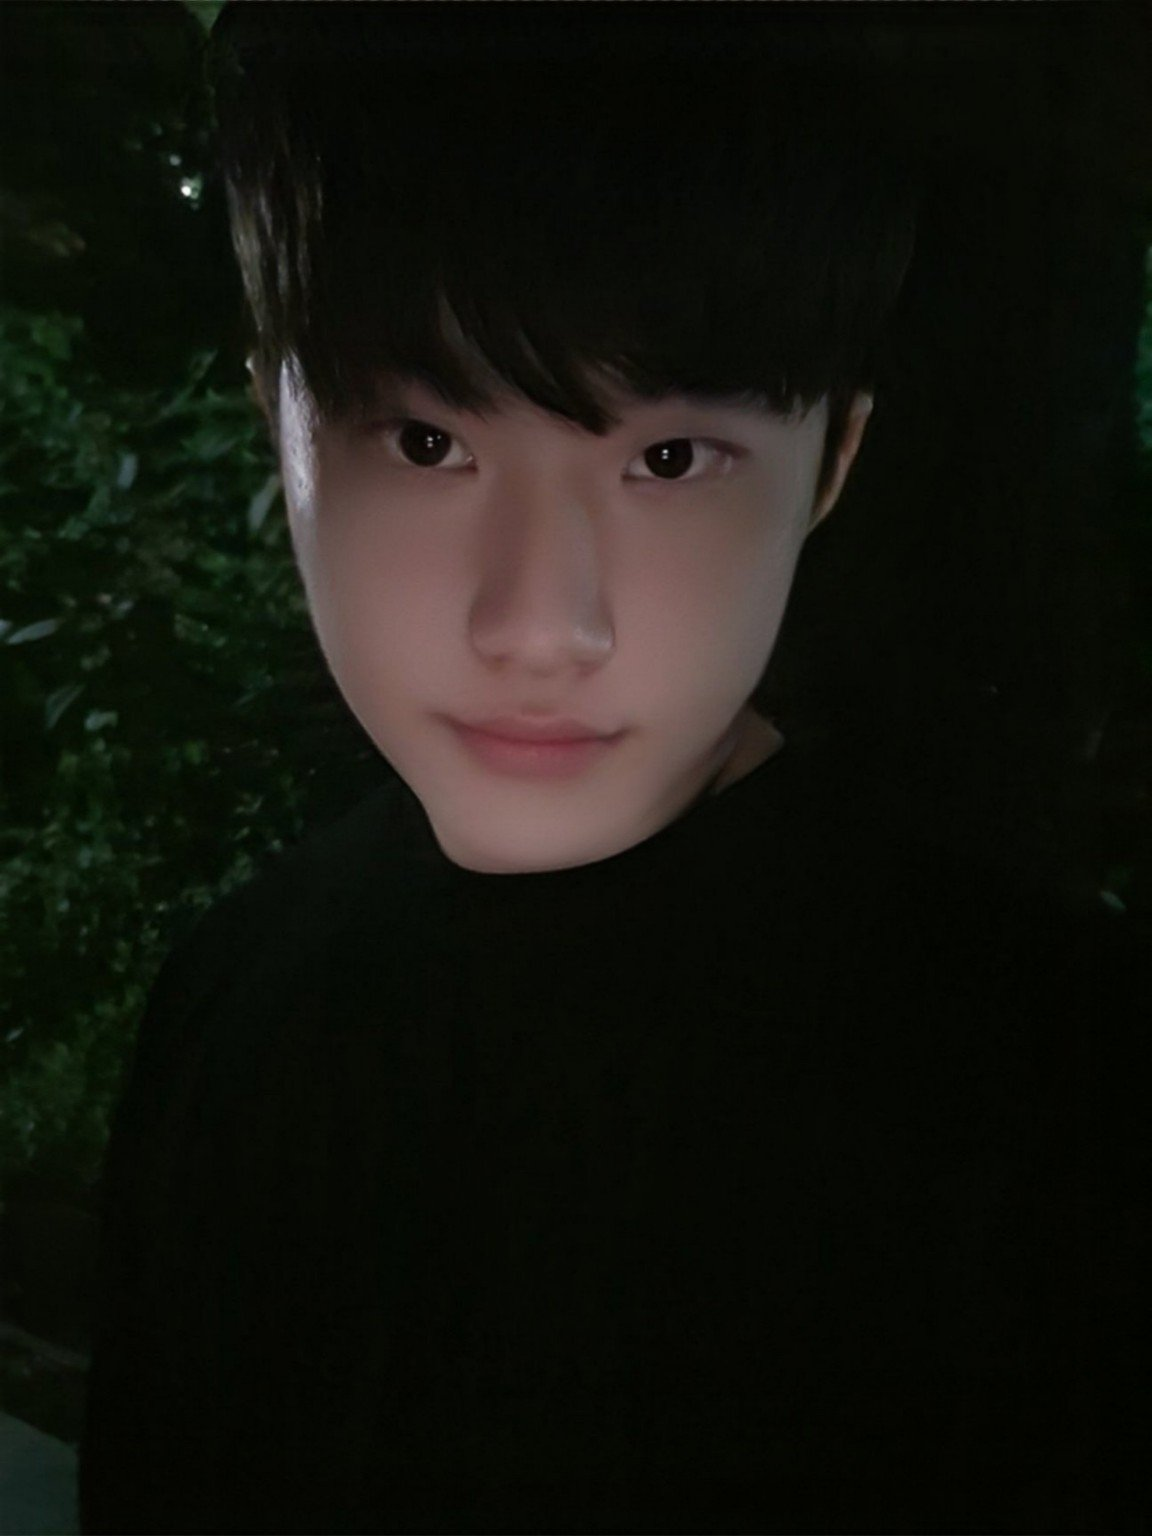
\includegraphics[width=3.2cm]{photo.jpg}
\end{minipage}%
\hfill
\begin{minipage}[c]{0.75\textwidth}
  \begin{center}
    {\LARGE\bfseries Jungseob Lee} \\[6pt]
    {\color{lighttext} NLP Researcher $\cdot$ Graduate Student, Korea University} \\[10pt]
    \begin{tabular}{ccc}
      \faIcon{birthday-cake}~1995.10.11 &
      \faIcon{envelope}~\href{mailto:omanma1928@korea.ac.kr}{omanma1928@korea.ac.kr} &
      \faIcon{globe}~\href{https://js-lee-ai.github.io}{js-lee-ai.github.io} \\[3pt]
      \faIcon{github}~\href{https://github.com/js-lee-AI}{js-lee-AI} &
      \faIcon{linkedin}~\href{https://www.linkedin.com/in/jslee-nlp/}{LinkedIn} &
      \faIcon{graduation-cap}~\href{https://scholar.google.com/citations?hl=ko&user=dTBGyFIAAAAJ}{Google Scholar}
    \end{tabular}
  \end{center}
\end{minipage}

\vspace{4pt}

% ═══════════════════════════════════════════
%  Summary
% ═══════════════════════════════════════════
\section{Summary}
Integrated M.S./Ph.D. researcher at Korea University NLP Lab (Advisor: Prof.~Heuiseok Lim), working on large language models and natural language processing --- agentic LLMs, efficient reasoning, machine translation, information retrieval, and model merging. First-author work at \textbf{EMNLP 2026} (Main), \textbf{ACL 2025} (Oral), and \textbf{Findings of ACL 2024}; four papers accepted at \textbf{EMNLP 2026} (2 Main, 2 Findings). Served as post-training Project Manager (Korea University representative) for \textbf{VAETKI}, Korea's sovereign foundation model.
\vspace{3pt}\\
\textbf{Research Interests:} Large Language Models, Agentic LLM, Efficient Reasoning, Machine Translation, Information Retrieval, Model Merging

% ═══════════════════════════════════════════
%  Education
% ═══════════════════════════════════════════
\section{Education}
\cventry{Integrated M.S./Ph.D. in Computer Science}{2021 -- Present}{Korea University, Seoul, Korea}{\textbf{Expected: Feb. 2027}}
\begin{itemize}
  \item NLP Lab, Advisor: Prof.~Heuiseok Lim --- large language models, agentic LLM, efficient reasoning, machine translation, information retrieval, and model merging
\end{itemize}

% ═══════════════════════════════════════════
%  Research Experience
% ═══════════════════════════════════════════
\section{Research Experience}

\textbf{VAETKI --- Korean Sovereign AI Foundation Model} \hfill \textit{Jun 2025 -- Jan 2026} \\
\textit{Post-training Project Manager --- Korea University Representative} \hfill {\footnotesize\color{lighttext} NC AI (NCSOFT)-led consortium} \\[2pt]
\begin{itemize}
  \item Led the post-training pipeline (SFT, RL, dataset curation) as PM for Korea University; selected by the Ministry of Science and ICT for Korea's national Sovereign AI Foundation Model program (NC AI-led 14-institution consortium; open-sourced Dec 2025).
  \item State-of-the-art on Korean language/culture (CLIcK), reasoning (KoBALT), professional knowledge (KMMLU-Pro), and instruction following (IFEval).
  \item \href{https://huggingface.co/NC-AI-consortium-VAETKI/VAETKI}{[\textcolor{accent}{Model}]} \enspace \href{https://github.com/wbl-ncai/VAETKI/blob/releases/v1.0.0/VAETKI_Technical_Report.pdf}{[\textcolor{accent}{Technical Report}]}
\end{itemize}
\vspace{5pt}

\textbf{Cross-lingual Language Transfer for Large Language Models} \hfill \textit{2024 -- 2025} \\
\textit{Lead Researcher (first author)} \hfill {\footnotesize\color{lighttext} Published at ACL 2025 (Oral)} \\[2pt]
\begin{itemize}
  \item Cross-lingual optimization that transfers English-centric LLMs to new languages while preserving source-language ability; \textbf{Oral} at ACL 2025.
  \item \href{https://aclanthology.org/2025.acl-long.734.pdf}{[\textcolor{accent}{PDF}]}
\end{itemize}
\vspace{5pt}

\textbf{Length-aware Byte Pair Encoding for Korean Machine Translation} \hfill \textit{2024} \\
\textit{Lead Researcher (first author)} \hfill {\footnotesize\color{lighttext} Published at Findings of ACL 2024} \\[2pt]
\begin{itemize}
  \item Length-aware BPE tokenization that mitigates over-segmentation in Korean machine translation and improves translation quality; \textbf{Findings of ACL 2024}.
  \item \href{https://aclanthology.org/2024.findings-acl.135.pdf}{[\textcolor{accent}{PDF}]}
\end{itemize}

% ═══════════════════════════════════════════
%  Awards
% ═══════════════════════════════════════════
\section{Awards}
\textbf{Best Paper Award (Top 1)} \hfill \textit{2025} \\
Annual Conference on Human and Cognitive Language Technology (HCLT 2025) \\[2pt]
{\small For \papertitle{KULLM-RAG: A RAG-Specialized Large Language Model with Intelligent Self-Verification}; \me{J.~Lee} (first author), M.~Kim, J.~Yoon, \textit{et al.} --- Korea University, Soongsil University, Human-Inspired AI Research.}

% ═══════════════════════════════════════════
%  Publications
% ═══════════════════════════════════════════
\section{Publications}
{\small\color{lighttext} \underline{Underlined} = me; $^{*}$ equal contribution. Full list (31 papers) on \href{https://scholar.google.com/citations?hl=ko&user=dTBGyFIAAAAJ}{\textcolor{accent}{Google Scholar}}.}
\vspace{4pt}

{\color{accent}\textbf{2026}}
\begin{itemize}
  \item \papertitle{The Geometry of Hallucination Detection: Why Simple Probes Are Sufficient} ---
    \me{J.~Lee}, J.~Seo, H.~Lim ~\textbf{EMNLP 2026} (Main)
  \item \papertitle{Language Chain in Alignment: Cross-Lingual Ranking Preference Optimization} ---
    S.~Lee, M.~Kim, \me{J.~Lee}, H.~Lim ~\textbf{EMNLP 2026} (Main)
  \item \papertitle{DART: Draft-Agreement Routing for Training-Free Adaptive Thinking Budgets in Hybrid Reasoning Models} ---
    \me{J.~Lee}, S.~Hong, S.~Lee, \textit{et al.} ~\textbf{Findings of EMNLP 2026} ~\href{https://arxiv.org/abs/2606.23181}{[\textcolor{accent}{arXiv}]}
  \item \papertitle{ThinkFuse: Trajectory-Aware Test-Time Fusion for Small Reasoning Models} ---
    M.~Kang$^{*}$, \me{J.~Lee}$^{*}$, J.~Seo, H.~Lim ~\textbf{Findings of EMNLP 2026}
  \item \papertitle{Improving Semantic Proximity in Information Retrieval through Cross-Lingual Alignment} ---
    S.~Hong, Y.~Jang, \me{J.~Lee}, H.~Moon, H.~Lim ~\textbf{ICLR 2026} (Poster) ~\paperlink{https://openreview.net/pdf?id=NvKvW5k6Kk}
  \item \papertitle{Towards Enhancing Natural Language Inference for Identifying Erroneous Outputs in Data-to-Text Generation} ---
    C.~Ok, E.K.~Lee, H.~Ju, \me{J.~Lee}, D.~Oh ~\textbf{Knowledge-Based Systems} ~\doilink{https://www.sciencedirect.com/science/article/pii/S0950705126006878}
  \item \papertitle{Beyond Penalizing Mistakes: Stabilizing Efficiency Training in Large Reasoning Models via Adaptive Correct-Only Rewards} ---
    \me{J.~Lee}, S.~Lee, S.~Hong, M.~Kim, C.~Park, H.~Lim ~Preprint ~\href{https://arxiv.org/abs/2606.22716}{[\textcolor{accent}{arXiv}]}
  \item \papertitle{To Isolate or to Score? Model-Adaptive Assessment for Cost-Efficient Multi-Agent RAG} ---
    \me{J.~Lee}, C.~Park, H.~Lim ~Preprint ~\href{https://arxiv.org/abs/2606.25191}{[\textcolor{accent}{arXiv}]}
  \item \papertitle{Skin-Deep: A Geometric Diagnostic for Alignment Fragility in LLM Representations} ---
    D.J.~Lee$^{*}$, \me{J.~Lee}$^{*}$, S.~Lee, \textit{et al.} ~Preprint ~\href{https://arxiv.org/abs/2606.22676}{[\textcolor{accent}{arXiv}]}
\end{itemize}

{\color{accent}\textbf{2025}}
\begin{itemize}
  \item \papertitle{Cross-lingual Optimization for Language Transfer in Large Language Models} ---
    \me{J.~Lee}, S.~Hong, H.~Moon, H.S.~Lim ~\textbf{ACL 2025} (Oral) ~\paperlink{https://aclanthology.org/2025.acl-long.734.pdf}
  \item \papertitle{An Analysis on Language Transfer of Pre-trained Language Model with Cross-lingual Post-training} ---
    S.~Son, C.~Park, \me{J.~Lee}, \textit{et al.} ~\textbf{Expert Systems with Applications} ~\doilink{https://doi.org/10.1016/j.eswa.2024.125841}
\end{itemize}

{\color{accent}\textbf{2024}}
\begin{itemize}
  \item \papertitle{Length-aware Byte Pair Encoding for Mitigating Over-segmentation in Korean Machine Translation} ---
    \me{J.~Lee}, H.~Moon, S.~Lee, C.~Park, S.~Eo, \textit{et al.} ~\textbf{Findings of ACL 2024} ~\paperlink{https://aclanthology.org/2024.findings-acl.135.pdf}
  \item \papertitle{Analysis of Model-, Data-, and User-Centric Approaches for Chat Applications: A Case Study of BlenderBot 2.0} ---
    C.~Park, \me{J.~Lee}, S.~Son, \textit{et al.} ~\textbf{Applied Sciences} ~\doilink{https://doi.org/10.3390/app14114821}
\end{itemize}

{\color{accent}\textbf{2023}}
\begin{itemize}
  \item \papertitle{A Survey on Evaluation Metrics for Machine Translation} ---
    S.~Lee, \me{J.~Lee}, H.~Moon, \textit{et al.} ~\textbf{Mathematics} (142 citations) ~\paperlink{https://www.mdpi.com/2227-7390/11/4/1006}
  \item \papertitle{PEEP-Talk: A Situational Dialogue-based Chatbot for English Education} ---
    S.~Lee, Y.~Jang, C.~Park, \me{J.~Lee}, \textit{et al.} ~\textbf{ACL 2023} (Demo) ~\paperlink{https://aclanthology.org/2023.acl-demo.18.pdf}
\end{itemize}

{\color{accent}\textbf{2022}}
\begin{itemize}
  \item \papertitle{QUAK: A Synthetic Quality Estimation Dataset for Korean-English Neural Machine Translation} ---
    S.~Eo, C.~Park, H.~Moon, J.~Seo, G.~Kim, \me{J.~Lee}, H.S.~Lim ~\textbf{COLING 2022} ~\paperlink{https://aclanthology.org/2022.coling-1.460.pdf}
  \item \papertitle{K-NCT: Korean Neural Grammatical Error Correction Gold-standard Test Set} ---
    S.~Koo, C.~Park, J.~Seo, S.~Lee, H.~Moon, \me{J.~Lee}, H.~Lim ~\textbf{IEEE Access} ~\paperlink{https://ieeexplore.ieee.org/document/9938990}
\end{itemize}

\vfill
\begin{center}
  \color{lighttext}\footnotesize Last updated: \today
\end{center}

\end{document}
